\documentclass{standalone}
\usepackage{tikz}
\usetikzlibrary{patterns, positioning}


\begin{document}
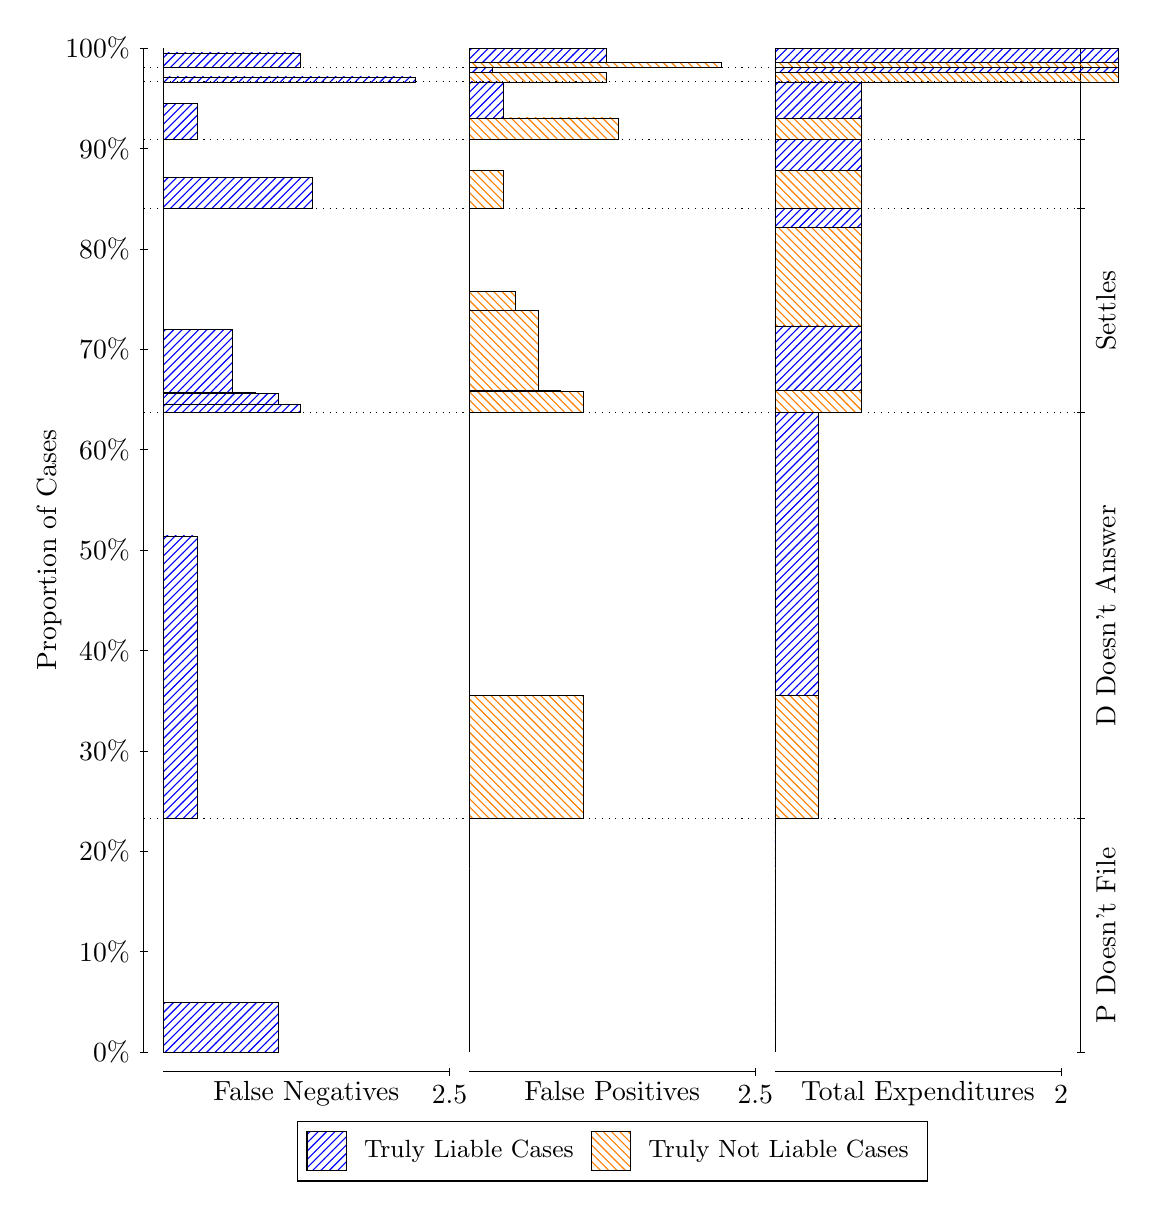
\begin{tikzpicture}
\draw[black, very thin] (1.5,1.75) -- (1.5,14.5);
\node[rotate=90, text=black, anchor=center] at (0.3, 8.125) {Proportion of Cases};
\draw[black, very thin] (1.45,1.75) -- (1.55,1.75);
\node[text=black, anchor=east] at (1.45, 1.75) {0\%};
\draw[black, very thin] (1.45,3.025) -- (1.55,3.025);
\node[text=black, anchor=east] at (1.45, 3.025) {10\%};
\draw[black, very thin] (1.45,4.3) -- (1.55,4.3);
\node[text=black, anchor=east] at (1.45, 4.3) {20\%};
\draw[black, very thin] (1.45,5.575) -- (1.55,5.575);
\node[text=black, anchor=east] at (1.45, 5.575) {30\%};
\draw[black, very thin] (1.45,6.85) -- (1.55,6.85);
\node[text=black, anchor=east] at (1.45, 6.85) {40\%};
\draw[black, very thin] (1.45,8.125) -- (1.55,8.125);
\node[text=black, anchor=east] at (1.45, 8.125) {50\%};
\draw[black, very thin] (1.45,9.4) -- (1.55,9.4);
\node[text=black, anchor=east] at (1.45, 9.4) {60\%};
\draw[black, very thin] (1.45,10.675) -- (1.55,10.675);
\node[text=black, anchor=east] at (1.45, 10.675) {70\%};
\draw[black, very thin] (1.45,11.95) -- (1.55,11.95);
\node[text=black, anchor=east] at (1.45, 11.95) {80\%};
\draw[black, very thin] (1.45,13.225) -- (1.55,13.225);
\node[text=black, anchor=east] at (1.45, 13.225) {90\%};
\draw[black, very thin] (1.45,14.5) -- (1.55,14.5);
\node[text=black, anchor=east] at (1.45, 14.5) {100\%};

\draw[black, very thin] (13.4,1.75) -- (13.4,14.5);
\draw[black, very thin] (13.35,1.75) -- (13.45,1.75);
\node[anchor=west] at (13.35, 1.75) {};
\draw[black, very thin] (13.35,4.7119) -- (13.45,4.7119);
\node[anchor=west] at (13.35, 4.7119) {};
\draw[black, very thin] (13.35,9.8679) -- (13.45,9.8679);
\node[anchor=west] at (13.35, 9.8679) {};
\draw[black, very thin] (13.35,12.463) -- (13.45,12.463);
\node[anchor=west] at (13.35, 12.463) {};
\draw[black, very thin] (13.35,13.344) -- (13.45,13.344);
\node[anchor=west] at (13.35, 13.344) {};
\draw[black, very thin] (13.35,14.07) -- (13.45,14.07);
\node[anchor=west] at (13.35, 14.07) {};
\draw[black, very thin] (13.35,14.258) -- (13.45,14.258);
\node[anchor=west] at (13.35, 14.258) {};
\draw[black, very thin] (13.35,14.5) -- (13.45,14.5);
\node[anchor=west] at (13.35, 14.5) {};

\draw[black, very thin, pattern color=blue, pattern=north east lines] (1.75,1.75) rectangle (3.2033,2.3803);
\draw[black, very thin, pattern color=orange, pattern=north west lines] (1.75,2.3803) rectangle (1.75,4.7119);
\draw[black, very thin, pattern color=blue, pattern=north east lines] (1.75,4.7119) rectangle (2.186,8.3031);
\draw[black, very thin, pattern color=orange, pattern=north west lines] (1.75,8.3031) rectangle (1.75,9.8679);
\draw[black, very thin, pattern color=blue, pattern=north east lines] (1.75,9.8679) rectangle (3.494,9.9779);
\draw[black, very thin, pattern color=blue, pattern=north east lines] (1.75,9.9779) rectangle (3.2033,10.11);
\draw[black, very thin, pattern color=blue, pattern=north east lines] (1.75,10.11) rectangle (2.9127,10.128);
\draw[black, very thin, pattern color=blue, pattern=north east lines] (1.75,10.128) rectangle (2.622,10.926);
\draw[black, very thin, pattern color=orange, pattern=north west lines] (1.75,10.926) rectangle (1.75,12.463);
\draw[black, very thin, pattern color=blue, pattern=north east lines] (1.75,12.463) rectangle (3.6393,12.861);
\draw[black, very thin, pattern color=orange, pattern=north west lines] (1.75,12.861) rectangle (1.75,13.344);
\draw[black, very thin, pattern color=blue, pattern=north east lines] (1.75,13.344) rectangle (2.186,13.799);
\draw[black, very thin, pattern color=orange, pattern=north west lines] (1.75,13.799) rectangle (1.75,14.07);
\draw[black, very thin, pattern color=blue, pattern=north east lines] (1.75,14.07) rectangle (4.9473,14.133);
\draw[black, very thin, pattern color=orange, pattern=north west lines] (1.75,14.133) rectangle (1.75,14.258);
\draw[black, very thin, pattern color=blue, pattern=north east lines] (1.75,14.258) rectangle (3.494,14.437);
\draw[black, very thin, pattern color=orange, pattern=north west lines] (1.75,14.437) rectangle (1.75,14.5);
\draw[black, very thin, pattern color=orange, pattern=north west lines] (5.6333,1.75) rectangle (5.6333,4.0815);
\draw[black, very thin, pattern color=blue, pattern=north east lines] (5.6333,4.0815) rectangle (5.6333,4.7119);
\draw[black, very thin, pattern color=orange, pattern=north west lines] (5.6333,4.7119) rectangle (7.0867,6.2766);
\draw[black, very thin, pattern color=blue, pattern=north east lines] (5.6333,6.2766) rectangle (5.6333,9.8679);
\draw[black, very thin, pattern color=orange, pattern=north west lines] (5.6333,9.8679) rectangle (7.0867,10.135);
\draw[black, very thin, pattern color=orange, pattern=north west lines] (5.6333,10.135) rectangle (6.796,10.154);
\draw[black, very thin, pattern color=orange, pattern=north west lines] (5.6333,10.154) rectangle (6.5053,11.17);
\draw[black, very thin, pattern color=orange, pattern=north west lines] (5.6333,11.17) rectangle (6.2147,11.405);
\draw[black, very thin, pattern color=blue, pattern=north east lines] (5.6333,11.405) rectangle (5.6333,12.463);
\draw[black, very thin, pattern color=orange, pattern=north west lines] (5.6333,12.463) rectangle (6.0693,12.946);
\draw[black, very thin, pattern color=blue, pattern=north east lines] (5.6333,12.946) rectangle (5.6333,13.344);
\draw[black, very thin, pattern color=orange, pattern=north west lines] (5.6333,13.344) rectangle (7.5227,13.614);
\draw[black, very thin, pattern color=blue, pattern=north east lines] (5.6333,13.614) rectangle (6.0693,14.07);
\draw[black, very thin, pattern color=orange, pattern=north west lines] (5.6333,14.07) rectangle (7.3773,14.195);
\draw[black, very thin, pattern color=blue, pattern=north east lines] (5.6333,14.195) rectangle (5.924,14.258);
\draw[black, very thin, pattern color=orange, pattern=north west lines] (5.6333,14.258) rectangle (8.8307,14.321);
\draw[black, very thin, pattern color=blue, pattern=north east lines] (5.6333,14.321) rectangle (7.3773,14.5);
\draw[black, very thin, pattern color=orange, pattern=north west lines] (9.5167,1.75) rectangle (9.5167,4.0815);
\draw[black, very thin, pattern color=blue, pattern=north east lines] (9.5167,4.0815) rectangle (9.5167,4.7119);
\draw[black, very thin, pattern color=orange, pattern=north west lines] (9.5167,4.7119) rectangle (10.062,6.2766);
\draw[black, very thin, pattern color=blue, pattern=north east lines] (9.5167,6.2766) rectangle (10.062,9.8679);
\draw[black, very thin, pattern color=orange, pattern=north west lines] (9.5167,9.8679) rectangle (10.607,10.154);
\draw[black, very thin, pattern color=blue, pattern=north east lines] (9.5167,10.154) rectangle (10.607,10.97);
\draw[black, very thin, pattern color=orange, pattern=north west lines] (9.5167,10.97) rectangle (10.607,12.221);
\draw[black, very thin, pattern color=blue, pattern=north east lines] (9.5167,12.221) rectangle (10.607,12.463);
\draw[black, very thin, pattern color=orange, pattern=north west lines] (9.5167,12.463) rectangle (10.607,12.946);
\draw[black, very thin, pattern color=blue, pattern=north east lines] (9.5167,12.946) rectangle (10.607,13.344);
\draw[black, very thin, pattern color=orange, pattern=north west lines] (9.5167,13.344) rectangle (10.607,13.614);
\draw[black, very thin, pattern color=blue, pattern=north east lines] (9.5167,13.614) rectangle (10.607,14.07);
\draw[black, very thin, pattern color=orange, pattern=north west lines] (9.5167,14.07) rectangle (13.877,14.195);
\draw[black, very thin, pattern color=blue, pattern=north east lines] (9.5167,14.195) rectangle (13.877,14.258);
\draw[black, very thin, pattern color=orange, pattern=north west lines] (9.5167,14.258) rectangle (13.877,14.321);
\draw[black, very thin, pattern color=blue, pattern=north east lines] (9.5167,14.321) rectangle (13.877,14.5);
\draw[black, dotted] (1.5,4.7119) -- (13.4,4.7119);
\draw[black, dotted] (1.5,9.8679) -- (13.4,9.8679);
\draw[black, dotted] (1.5,12.463) -- (13.4,12.463);
\draw[black, dotted] (1.5,13.344) -- (13.4,13.344);
\draw[black, dotted] (1.5,14.07) -- (13.4,14.07);
\draw[black, dotted] (1.5,14.258) -- (13.4,14.258);
\draw[black, very thin] (1.75,1.5) -- (5.3833,1.5);
\node[text=black, anchor=north] at (3.5667, 1.5) {False Negatives};
\draw[black, very thin] (5.3833,1.45) -- (5.3833,1.55);
\node[text=black, anchor=north] at (5.3833, 1.45) {2.5};

\draw[black, very thin] (5.6333,1.5) -- (9.2667,1.5);
\node[text=black, anchor=north] at (7.45, 1.5) {False Positives};
\draw[black, very thin] (9.2667,1.45) -- (9.2667,1.55);
\node[text=black, anchor=north] at (9.2667, 1.45) {2.5};

\draw[black, very thin] (9.5167,1.5) -- (13.15,1.5);
\node[text=black, anchor=north] at (11.333, 1.5) {Total Expenditures};
\draw[black, very thin] (13.15,1.45) -- (13.15,1.55);
\node[text=black, anchor=north] at (13.15, 1.45) {2};

\node[text=black, centered, rotate=90] at (13.72, 3.2309) {P Doesn't File};
\node[text=black, centered, rotate=90] at (13.72, 7.2899) {D Doesn't Answer};
\node[text=black, centered, rotate=90] at (13.72, 11.165) {Settles};





\draw (7.449999999999999,1.5) node[draw=none] (baseCoordinate) {};
\begin{scope}[align=center]
        \matrix[scale=0.5, draw=black, below=0.5cm of baseCoordinate, nodes={draw}, column sep=0.1cm]{
            \node[rectangle, draw, minimum width=0.5cm, minimum height=0.5cm, pattern color=blue, pattern=north east lines] {}; &
            \node[draw=none, font=\small, text=black] (B) {Truly Liable Cases}; &
            \node[rectangle, draw, minimum width=0.5cm, minimum height=0.5cm, pattern color=orange, pattern=north west lines] {}; &
            \node[draw=none, font=\small, text=black] (B) {Truly Not Liable Cases}; \\
            };
\end{scope}

\end{tikzpicture}
\end{document}